\chapter{Présentation d'ORESM}
\og \textit{Nous devons espérer (...) que l'autorité publique prendra quelque jour les mesures nécessaires pour concentrer définitivement, du moins autant que possible, ces documents, qui perdent par leur dispersion une grande partie de leur valeur, et pour mettre fin à un état des choses aussi contraire à la loi qu'à l'intérêt des lettres.}\fg  Auguste Vallet de Virville\footnote{Archiviste et historien français né en 1815 et mort en 1868.}, \textit{Histoire de l'instruction publique en Europe et principalement en France, depuis le christianisme jusqu'à nos jours}, 1849.
\section{Origine}
On ne peut pas dissocier le projet ORESM (Œuvres et Référentiels des étudiants, Suppôts et Maîtres) de \textit{Studium Parisiense}\footnote{\href{http://studium.univ-paris1.fr/}{http://studium.univ-paris1.fr/}} qui est une base de données prosopo-bio-bibliographique. Initialement débuté comme un projet pédagogique dans les années 1970, il enseignait aux élèves la construction d'une base de données à partir de leurs propres dépouillements de répertoires biographiques. Au fil des années la masse des données s'est alourdie pour arriver à près de 20 000 fiches. C'est en 2019, quand Jean-Philippe Genet\footnote{Médiéviste spécialiste de l’Angleterre et professeur émérite d’histoire médiévale à la Sorbonne.} initie la restructuration de la base de données \textit{Studium Parisiense}, que débute la réflexion qui débouchera au projet ORESM. Il émet la volonté de valoriser son gisement de données en rendant ces données consultables et utilisables. Pour réfléchir aux différents moyens et formes qui peuvent être mis en œuvre, la BIS recrute pour un stage de quatre mois Lucie Vieillon étudiante du master \og\textit{Technologiques numériques appliquées à l'histoire}\fg. Au cours de cette période elle va participer à la rédaction d'un dossier de demande de financement dans le cadre de l'appel à projets Collex Persée, qui conduira à une première définition des objectifs du projet ORESM. Il est alors proposé de mettre en valeur les données prosopographiques venant de \textit{Studium Parisiense} et les données patrimoniales issues des archives de l'université sur un unique portail web. On permettrait ainsi aux chercheurs de bénéficier d'un unique point d'accès pour se retrouver dans le contenu des différentes institutions possédant des archives de l'université. 
\par
La dispersion des archives relatives à l'université de Paris n'est pas récente. En effet à la Révolution française il y a une volonté de regrouper les fonds d'archives du clergé aux Archives nationales,  suivant la loi du 7 messidor de l'an II. Cette volonté est exécutée de manière partielle se concentrant principalement sur les archives domaniales et laissant éparpillées un grand nombre d'archives relatives à l'université dans différentes institutions comme le collège Louis-le-Grand, l'Hôtel de ville, la bibliothèques Mazarine etc. L'envie de regrouper les archives de l'ancienne université va émerger au cours du siècle suivant. En 1837, Auguste Vallet de Viriville a été chargé par François Guizot\footnote{Homme d'état français. Né en 1787 et mort en 1874, il est important dans l'histoire de l'éducation en France, principalement pour la loi de 1833 qui porte son nom, qui impose à chaque commune de plus de 500 habitants d'avoir une école primaire.} de mettre en ordre les archives de l'ancienne université de Paris. Il a intégré dans le fonds des registres qui étaient restés en possession de la bibliothèque de la Sorbonne. Au fur et à mesure des regroupements successifs du \textsc{XIX}\ieme{} siècle le nombre d'institutions en possession d'archives relatives à l'université de Paris se réduit pour n'être finalement de nos jours plus que la BIS et les Archives nationales, en majorité, ainsi que la Bibliothèque interuniversitaire de Santé (BIUS).
\par
\begin{figure}[!h]
    \centering
    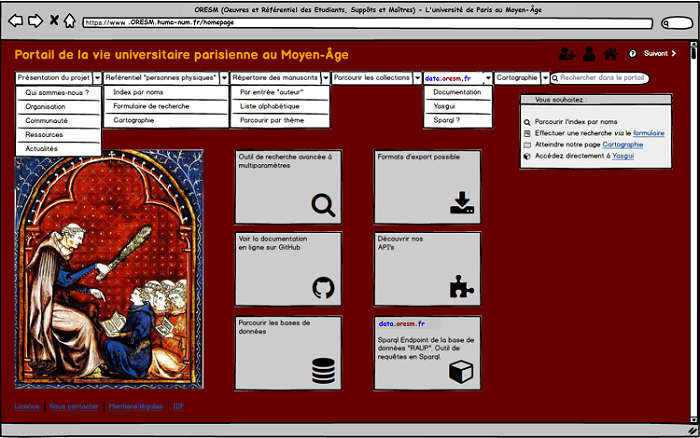
\includegraphics[width=1\linewidth]{images/oresm origine.png}
    \caption{Maquette présentant l'idée initiale du portail ORESM.}
    \label{fig:oresm-origine}
\end{figure}
Finalement il avait été décidé que le projet ORESM se composerait de plusieurs réalisations accessibles par le portail web centralisateur. Un inventaire virtuel regroupant les différentes notices des archives concernant l'université sur la période étudiée, un référentiel des personnes liées à celle-ci, un répertoire des manuscrits, les données contenues dans ces trois composants étant par ailleurs agrégées ou rendues accessibles via une base de données. Plus récemment le projet ORESM a prévu d'ajouter une corde d'édition numérique à son arc avec le projet ECRU (éditions critiques relatives à l’Université de Paris), annexe du projet ORESM, qui vise à encoder des éditions critiques d'actes à l'aide de l'IA\footnote{\og Intelligence Artificielle\fg  Ensemble de théories et de techniques mises en œuvre en vue de réaliser des machines capables de simuler l'intelligence humaine.}. L'encodage se fera en XML-TEI. L'innovation de cette approche réside dans le corpus qui est en latin, aucun autre projet n'avait utilisé l'IA pour réaliser un balisage automatique sur du texte en latin. Les éditions sont tirées des grands ouvrages relatifs aux archives de l'université de Paris en commençant par le \og \textit{Chartularium Universitatis Parisiensis}\fg d’Heinrich Denifle et Emile Châtelain. Le projet ECRU est à ses débuts mais il enrichira à terme les référentiels et la base de données d'ORESM notamment concernant les entités nommées.
\section{Les acteurs}
\subsection{La BIS}
La BIS porte le projet à partir de son service le SERVAL (Service de la Valorisation numérique des collections et du soutien à la Recherche). Son nom est assez explicite concernant sa vocation. Avec les outils numériques disponibles le SERVAL va réaliser des projets de valorisation de sources historiques touchant de près ou de loin à la vie universitaire parisienne. Comme autres projets actuellement portés nous pouvons citer \og ès lettres\fg\footnote{\href{https://www.collexpersee.eu/projet/es-lettres/}{https://www.collexpersee.eu/projet/es-lettres/}} qui porte sur la numérisation et la valorisation des thèses françaises du \textsc{XIX}\ieme{} siècle avec une exposition virtuelle\footnote{\href{https://nubis.univ-paris1.fr/s/theses-doctorats-es-lettres-19-siecle-exposition-devenir-savant/page/introduction}{Lien vers cette exposition virtuelle}}, et une base de données. Nous pouvons également citer le projet PRET19 \footnote{Projet de Répertoire des Emprunteurs et Titres empruntés au \textsc{XIX}\ieme{} siècle à l’université \href{https://www.collexpersee.eu/projet/pret19/}{https://www.collexpersee.eu/projet/pret19/}} qui numérise les registres de prêt de plusieurs bibliothèques parisiennes en commençant au \textsc{XIX}\ieme{} siècle. En plus de cette numérisation le projet prévoit d'utiliser un OCR\footnote{\og Optical Character Recognition\fg  Procédé qui consiste à extraire automatiquement le texte d'une image numérique.} pour extraire des données des registres et construire une base de données accessible en ligne. Ces projets illustrent clairement la mission du SERVAL c'est à dire la production d'outils numériques qui serviront à alimenter la recherche sur des thèmes relatifs à l'histoire de l'université de Paris. Le projet ORESM à la BIS est actuellement dirigé par Laurence Bobis, directrice de la bibliothèque. L'équipe travaillant sur le projet est composée de Laurie Aoustet, adjointe de la cheffe du SERVAL, Arsène Georges et Sébastien Clément.
\subsection{Le LaMOP}
Le Laboratoire de Médiévistique Occidentale de Paris est co-porteur du projet. Crée en 1998 sous l'impulsion de plusieurs chercheurs dont Jean Philippe Genet, ce laboratoire est marqué par une approche pluridisciplinaire du Moyen Âge. Son identité réside dans une pratique historienne qui combine les sciences de l’érudition avec les sciences humaines et sociales, le tout accompagné d’une composante informatique fort bien ancrée. Actuellement composé d'environs 70 chercheurs cet acteur du projet représente le volet scientifique par la voix de Thierry Kouamé\footnote{Professeur d’histoire médiévale à l’université de Franche-Comté. Ses recherches portent sur l’histoire sociale, politique et culturelle des institutions d’enseignement de l’Occident médiéval et sur les objets et méthodes de la prosopographie.} qui est co-directeur d'ORESM. C'est le LaMOP qui a repris \textit{Studium Parisiense} et qui poursuit son développement avec Stéphane Lamassé\footnote{Maître de conférences en histoire, civilisation, archéologie et art des mondes anciens et médiévaux à l’université Paris I Panthéon-Sorbonne. Ses thèmes de recherche sont l’histoire des mathématiques et les humanités numériques.}. 
\subsection{Les Archives nationales}
Dernier acteur principal, les Archives nationales (AN)\footnote{\href{https://www.archives-nationales.culture.gouv.fr/}{https://www.archives-nationales.culture.gouv.fr/}} participent activement à l'avancement du projet. Créée en 1790 cette institution est incontournable par la richesse des fonds qu'elle conserve. Relevant du ministère de la Culture les AN sont proches des milieux universitaires, et très souvent des soutiens de poids pour la recherche historique. En ce qui concerne le projet ORESM, les AN apportent deux expertises nécessaires à la réalisation des objectifs définis. D'une part en tant que conservateur majeur des archives du domaine d'ORESM, le Département du Moyen Âge et de l’Ancien Régime (DMAAR) apporte une expertise archivistique importante, notamment en la personne de Jean François Moufflet qui est responsable des fonds concernés aux Archives nationales et de leur traitement, description incluse. D'autre part par le biais du Lab des AN\footnote{Le Lab est un service qui pilote la recherche et l'innovation numériques des Archives nationales et qui porte de nombreux projets dans ce domaine.}. Ce service apporte au projet une expertise technique relatives aux technologies d'encodage et de transformation des métadonnées archivistiques. C'est la responsable du Lab, Florence Clavaud, qui sert de référent technique au projet.